\documentclass[]{article}
\usepackage{lmodern}
\usepackage{setspace}
\setstretch{1}
\usepackage{amssymb,amsmath}
\usepackage{ifxetex,ifluatex}
\usepackage{fixltx2e} % provides \textsubscript
\ifnum 0\ifxetex 1\fi\ifluatex 1\fi=0 % if pdftex
  \usepackage[T1]{fontenc}
  \usepackage[utf8]{inputenc}
\else % if luatex or xelatex
  \ifxetex
    \usepackage{mathspec}
  \else
    \usepackage{fontspec}
  \fi
  \defaultfontfeatures{Ligatures=TeX,Scale=MatchLowercase}
\fi
% use upquote if available, for straight quotes in verbatim environments
\IfFileExists{upquote.sty}{\usepackage{upquote}}{}
% use microtype if available
\IfFileExists{microtype.sty}{%
\usepackage{microtype}
\UseMicrotypeSet[protrusion]{basicmath} % disable protrusion for tt fonts
}{}
\usepackage[margin=1in]{geometry}
\usepackage{hyperref}
\PassOptionsToPackage{usenames,dvipsnames}{color} % color is loaded by hyperref
\hypersetup{unicode=true,
            pdftitle={Fisheries example integrating FLR},
            pdfauthor={A. Bradley Duthie¹³, Jeremy J. Cusack¹, Isabel L. Jones¹, Jeroen Minderman¹, Erlend B. Nilsen², Rocío A. Pozo¹, O. Sarobidy Rakotonarivo¹, Bram Van Moorter², and Nils Bunnefeld¹},
            colorlinks=true,
            linkcolor=blue,
            citecolor=Blue,
            urlcolor=Blue,
            breaklinks=true}
\urlstyle{same}  % don't use monospace font for urls
\usepackage{natbib}
\bibliographystyle{apalike}
\usepackage{color}
\usepackage{fancyvrb}
\newcommand{\VerbBar}{|}
\newcommand{\VERB}{\Verb[commandchars=\\\{\}]}
\DefineVerbatimEnvironment{Highlighting}{Verbatim}{commandchars=\\\{\}}
% Add ',fontsize=\small' for more characters per line
\usepackage{framed}
\definecolor{shadecolor}{RGB}{248,248,248}
\newenvironment{Shaded}{\begin{snugshade}}{\end{snugshade}}
\newcommand{\KeywordTok}[1]{\textcolor[rgb]{0.13,0.29,0.53}{\textbf{{#1}}}}
\newcommand{\DataTypeTok}[1]{\textcolor[rgb]{0.13,0.29,0.53}{{#1}}}
\newcommand{\DecValTok}[1]{\textcolor[rgb]{0.00,0.00,0.81}{{#1}}}
\newcommand{\BaseNTok}[1]{\textcolor[rgb]{0.00,0.00,0.81}{{#1}}}
\newcommand{\FloatTok}[1]{\textcolor[rgb]{0.00,0.00,0.81}{{#1}}}
\newcommand{\ConstantTok}[1]{\textcolor[rgb]{0.00,0.00,0.00}{{#1}}}
\newcommand{\CharTok}[1]{\textcolor[rgb]{0.31,0.60,0.02}{{#1}}}
\newcommand{\SpecialCharTok}[1]{\textcolor[rgb]{0.00,0.00,0.00}{{#1}}}
\newcommand{\StringTok}[1]{\textcolor[rgb]{0.31,0.60,0.02}{{#1}}}
\newcommand{\VerbatimStringTok}[1]{\textcolor[rgb]{0.31,0.60,0.02}{{#1}}}
\newcommand{\SpecialStringTok}[1]{\textcolor[rgb]{0.31,0.60,0.02}{{#1}}}
\newcommand{\ImportTok}[1]{{#1}}
\newcommand{\CommentTok}[1]{\textcolor[rgb]{0.56,0.35,0.01}{\textit{{#1}}}}
\newcommand{\DocumentationTok}[1]{\textcolor[rgb]{0.56,0.35,0.01}{\textbf{\textit{{#1}}}}}
\newcommand{\AnnotationTok}[1]{\textcolor[rgb]{0.56,0.35,0.01}{\textbf{\textit{{#1}}}}}
\newcommand{\CommentVarTok}[1]{\textcolor[rgb]{0.56,0.35,0.01}{\textbf{\textit{{#1}}}}}
\newcommand{\OtherTok}[1]{\textcolor[rgb]{0.56,0.35,0.01}{{#1}}}
\newcommand{\FunctionTok}[1]{\textcolor[rgb]{0.00,0.00,0.00}{{#1}}}
\newcommand{\VariableTok}[1]{\textcolor[rgb]{0.00,0.00,0.00}{{#1}}}
\newcommand{\ControlFlowTok}[1]{\textcolor[rgb]{0.13,0.29,0.53}{\textbf{{#1}}}}
\newcommand{\OperatorTok}[1]{\textcolor[rgb]{0.81,0.36,0.00}{\textbf{{#1}}}}
\newcommand{\BuiltInTok}[1]{{#1}}
\newcommand{\ExtensionTok}[1]{{#1}}
\newcommand{\PreprocessorTok}[1]{\textcolor[rgb]{0.56,0.35,0.01}{\textit{{#1}}}}
\newcommand{\AttributeTok}[1]{\textcolor[rgb]{0.77,0.63,0.00}{{#1}}}
\newcommand{\RegionMarkerTok}[1]{{#1}}
\newcommand{\InformationTok}[1]{\textcolor[rgb]{0.56,0.35,0.01}{\textbf{\textit{{#1}}}}}
\newcommand{\WarningTok}[1]{\textcolor[rgb]{0.56,0.35,0.01}{\textbf{\textit{{#1}}}}}
\newcommand{\AlertTok}[1]{\textcolor[rgb]{0.94,0.16,0.16}{{#1}}}
\newcommand{\ErrorTok}[1]{\textcolor[rgb]{0.64,0.00,0.00}{\textbf{{#1}}}}
\newcommand{\NormalTok}[1]{{#1}}
\usepackage{graphicx,grffile}
\makeatletter
\def\maxwidth{\ifdim\Gin@nat@width>\linewidth\linewidth\else\Gin@nat@width\fi}
\def\maxheight{\ifdim\Gin@nat@height>\textheight\textheight\else\Gin@nat@height\fi}
\makeatother
% Scale images if necessary, so that they will not overflow the page
% margins by default, and it is still possible to overwrite the defaults
% using explicit options in \includegraphics[width, height, ...]{}
\setkeys{Gin}{width=\maxwidth,height=\maxheight,keepaspectratio}
\IfFileExists{parskip.sty}{%
\usepackage{parskip}
}{% else
\setlength{\parindent}{0pt}
\setlength{\parskip}{6pt plus 2pt minus 1pt}
}
\setlength{\emergencystretch}{3em}  % prevent overfull lines
\providecommand{\tightlist}{%
  \setlength{\itemsep}{0pt}\setlength{\parskip}{0pt}}
\setcounter{secnumdepth}{0}
% Redefines (sub)paragraphs to behave more like sections
\ifx\paragraph\undefined\else
\let\oldparagraph\paragraph
\renewcommand{\paragraph}[1]{\oldparagraph{#1}\mbox{}}
\fi
\ifx\subparagraph\undefined\else
\let\oldsubparagraph\subparagraph
\renewcommand{\subparagraph}[1]{\oldsubparagraph{#1}\mbox{}}
\fi

%%% Use protect on footnotes to avoid problems with footnotes in titles
\let\rmarkdownfootnote\footnote%
\def\footnote{\protect\rmarkdownfootnote}

%%% Change title format to be more compact
\usepackage{titling}

% Create subtitle command for use in maketitle
\newcommand{\subtitle}[1]{
  \posttitle{
    \begin{center}\large#1\end{center}
    }
}

\setlength{\droptitle}{-2em}
  \title{Fisheries example integrating FLR}
  \pretitle{\vspace{\droptitle}\centering\huge}
  \posttitle{\par}
\subtitle{GMSE: an R package for generalised management strategy evaluation
(Supporting Information 5)}
  \author{A. Bradley Duthie¹³, Jeremy J. Cusack¹, Isabel L. Jones¹, Jeroen
Minderman¹, Erlend B. Nilsen², Rocío A. Pozo¹, O. Sarobidy
Rakotonarivo¹, Bram Van Moorter², and Nils Bunnefeld¹}
  \preauthor{\centering\large\emph}
  \postauthor{\par}
  \predate{\centering\large\emph}
  \postdate{\par}
  \date{{[}1{]} Biological and Environmental Sciences, University of Stirling,
Stirling, UK {[}2{]} Norwegian Institute for Nature Research, Trondheim,
Norway {[}3{]}
\href{mailto:alexander.duthie@stir.ac.uk}{\nolinkurl{alexander.duthie@stir.ac.uk}}}


\begin{document}
\maketitle

\section{Integration and simulation with
fisheries}\label{integration-and-simulation-with-fisheries}

Early development of management strategy evaluation (MSE) models
originated in fisheries \citep{Polacheck1999, Smith1999, Sainsbury2000}.
Consequently, fisheries-focused software for MSE has been extensively
developed, including R libraries that focus on the management of species
of exceptional interest, such as the Atlantic Bluefin Tuna
(\emph{Thunnus thynnus})
\citep[\href{https://github.com/ICCAT/abft-mse/tree/master/R_package/ABTMSE}{ABFTMSE};][]{Carruthers2018, Carruthers2018a},
and Indian Ocean Bigeye (\emph{T. obesus}) and Yellowfin (\emph{T.
albacares}) Tuna
\citep[\href{https://github.com/pjumppanen/MSE-IO-BET-YFT}{MSE-IO-BET-YFT};][]{Kolody2016}.
The largest of all such libraries is the Fisheries Library in R
(\href{http://www.flr-project.org/}{FLR}), which includes an extensive
collection of tools targeted for fisheries science. The FLR library has
been used in over a hundred
\href{http://www.flr-project.org/\#publications}{publications}
\citep[recent publications
include][]{Jardim2018, Mackinson2018, Utizi2018}, and includes
\href{http://www.flr-project.org/doc/An_introduction_to_MSE_using_FLR.html}{an
MSE framework} for evaluating different harvest control rules.

\textless{}\textless{}\textless{}\textless{}\textless{}\textless{}\textless{}
HEAD As part of the \href{https://sti-cs.org/confoobio/}{ConFooBio}
project, a central focus of GMSE is on simulating the management of
animal populations of conservation interest, with a particular emphasis
on understanding conservation conflict; further development of GMSE is
expected to continue with this as a priority, further building upon the
decision-making algorithms of managers and users to better understand
how conflict arises and can be managed and mitigated. Hence, GMSE is not
intended as a substitute for packages such as
\href{http://www.flr-project.org/}{FLR}, but the integration of these
packages with GMSE could make use of GSME's current and future
simulation capabilities, and particularly the \href{}{genetic
algorithm}. Such integration might be possible using the
\texttt{gmse\_apply} function, which allows for \href{}{custom defined
submodels} to be used within the GMSE framework, and with default GMSE
submodels. Hence, GMSE might be especially useful for modelling the
management of fisheries under conditions of increasing competing
staleholder demands and conflicts. We do not attempt such an ambitious
project here, but instead show how such a project could be developed
through integration of \href{http://www.flr-project.org/}{FLR} and
\texttt{gmse\_apply}. ======= As part of the
\href{https://sti-cs.org/confoobio/}{ConFooBio} project, a central focus
of GMSE is on simulating the management of populations of conservation
interest, with a particular emphasis on understanding conservation
conflict; further development of GMSE is expected to continue with this
as a priority, further building upon the decision-making algorithms of
managers and users to better understand how conflict arises and can
potentially be resolved. Hence, GMSE is not intended as a substitute for
packages such as \href{http://www.flr-project.org/}{FLR}, but the
integration of these packages with GMSE could make use of GSME's current
and future simulation capabilities, and particularly the \href{}{genetic
algorithm}. Such integration might be possible using the
\texttt{gmse\_apply} function, which allows for \href{}{custom defined
submodels} to be used within the GMSE framework, and with default GMSE
submodels. Hence, GMSE might be especially useful for modelling the
management of fisheries under conditions of increasing harvesting
demands and stakeholder conflict. We do not attempt such an ambitious
project here, but instead show how such a project could be developed
through integration of \href{http://www.flr-project.org/}{FLR} and
\texttt{gmse\_apply}.
\textgreater{}\textgreater{}\textgreater{}\textgreater{}\textgreater{}\textgreater{}\textgreater{}
366b9295e25f74c310c7185eab57ad3e19bfa83c

Here we follow a
\href{http://www.flr-project.org/doc/Modelling_stock_recruitment_with_FLSR.html}{Modelling
Stock-Recruitment with FLSR} example, then integrate this example with
\texttt{gmse\_apply} to explore the behaviour of a number of simulated
fishers who are goal-driven to maximise their own harvest and a manager
that aims to keep the fish stocks at a predefined target level. The core
concept in GMSE is that manager can only incentivise fishers to harvest
less or more by varying the cost of fishing (through e.g.~taxes) given a
set manager budget; please note that the manager cannot force the fisher
to follow any policy. Based on the cost of fishing, the fisher can then
given their own budget decide whether to invest in fishing or keep the
budget. This concepts represents a nartural resource managmeent and
conservation conflict, where one party aims to maximise their livelihood
(fisher) and the other aims to keep a population at a sustainable level
and prevent it from going extinct. Importantly, the manager does not
have full control over fishers but can set policies to incentivise
sustainable behaviour. We emphasise that this example is provided only
as demonstration of how GMSE can potentially be integrated with already
developed fisheries models, and is not intended to make recommendations
for management in any population.

\section{\texorpdfstring{Integrating with the Fisheries Library in R
(\href{http://www.flr-project.org/}{FLR})}{Integrating with the Fisheries Library in R (FLR)}}\label{integrating-with-the-fisheries-library-in-r-flr}

The FLR toolset includes \href{http://www.flr-project.org/\#packages}{a
series of pacakges}, with several
\href{http://www.flr-project.org/doc/index.html}{tutorials} for using
them. For simplicity, we focus here on
\href{http://www.flr-project.org/doc/Modelling_stock_recruitment_with_FLSR.html}{a
model of stock recruitment} to be used as the population model in
\texttt{gmse\_apply}. This population model will use sample data and one
of the many available stock-recruitment models available in FLR, and a
custom function will be written to return a single value for stock
recruitment. Currently, \texttt{gmse\_apply} requires that submodels
return subfunction results either as scalar values or data frames that
are structured in the same way as GMSE submodels. But interpretation of
scalar values is left up to the user (e.g., population model results
could be interpreted as abundance or biomass; manager policy could be
interpreted as cost of harvesting or as total allowable catch). For
simplicity, the observation (i.e., estimation) model will simply be the
stock reported from the population model with error, and the manager
model will be a total allowable catch calculated from the
stock-recruitment relationship that accounts for the number of fishers
in the system. The user model, however, will employ the full power of
the default GMSE user function to simulate user actions. We first show
how a custom function can be made that applies the FLR toolset to a
population model.

\section{Modelling stock-recruitment for the population
model}\label{modelling-stock-recruitment-for-the-population-model}

Here we closely follow
\href{http://www.flr-project.org/doc/Modelling_stock_recruitment_with_FLSR.html}{a
tutorial from the FLR project}. To build the stock-recruitment model,
the \texttt{FLCore} package is needed \citep{Kell2007}.

\begin{Shaded}
\begin{Highlighting}[]
\KeywordTok{install.packages}\NormalTok{(}\KeywordTok{c}\NormalTok{(}\StringTok{"FLCore"}\NormalTok{), }\DataTypeTok{repos=}\StringTok{"http://flr-project.org/R"}\NormalTok{);}
\end{Highlighting}
\end{Shaded}

To start, we need to read in the \texttt{FLCore} and GMSE libraries.

\begin{Shaded}
\begin{Highlighting}[]
\KeywordTok{library}\NormalTok{(FLCore);}
\end{Highlighting}
\end{Shaded}

\begin{verbatim}
## Loading required package: lattice
\end{verbatim}

\begin{verbatim}
## FLCore (Version 2.6.7, packaged: 2018-04-17 09:12:42 UTC)
\end{verbatim}

\begin{Shaded}
\begin{Highlighting}[]
\KeywordTok{library}\NormalTok{(GMSE);}
\end{Highlighting}
\end{Shaded}

For a simplified example in GMSE, we will simulate the process of stock
recruitment over multiple time steps using an example stock-recruitment
model. The stock-recruitment model describes the relationship between
stock-recruitment and spawning stock biomass. The sample that we will
work from is a recreation of the North Sea Herring (\texttt{nsher})
dataset available in the \texttt{FLCore} package \citep{Kell2007}. This
data set includes recruitment and spawning stock biomass data between
1960 and 2004. First, we initialise an empty \texttt{FLSR} object and
read in the recreated herring data files from GMSE, which contains
recruitment (\texttt{rec.n}) and spawning stock biomass (\texttt{ssb.n})

\begin{Shaded}
\begin{Highlighting}[]
\NormalTok{newFL   <-}\StringTok{ }\KeywordTok{FLSR}\NormalTok{(); }\CommentTok{# Initialises the empty FLSR object}
\KeywordTok{data}\NormalTok{(nsher_data); }\CommentTok{#called from GMSE library rather than nsher from FLCore library}
\end{Highlighting}
\end{Shaded}

The recruitment (\texttt{rec.n}) and spawning stock biomass
(\texttt{ssb.n}) data need to be in the form of a vector, array, matrix
to use them with \texttt{FLQuant}. We will convert \texttt{rec.n} and
\texttt{ssb.n} into matrices.

\begin{Shaded}
\begin{Highlighting}[]
\NormalTok{rec.m        <-}\StringTok{ }\KeywordTok{as.matrix}\NormalTok{(rec.n);}
\NormalTok{ssb.m        <-}\StringTok{ }\KeywordTok{as.matrix}\NormalTok{(ssb.n);}
\end{Highlighting}
\end{Shaded}

We can then construct two \texttt{FLQuant} objects, specifying the
relevant years and units.

\begin{Shaded}
\begin{Highlighting}[]
\NormalTok{Frec.m       <-}\StringTok{ }\KeywordTok{FLQuant}\NormalTok{(rec.m, }\DataTypeTok{dimnames=}\KeywordTok{list}\NormalTok{(}\DataTypeTok{age=}\DecValTok{1}\NormalTok{, }\DataTypeTok{year =} \DecValTok{1960}\NormalTok{:}\DecValTok{2004}\NormalTok{));}
\NormalTok{Fssb.m       <-}\StringTok{ }\KeywordTok{FLQuant}\NormalTok{(ssb.m, }\DataTypeTok{dimnames=}\KeywordTok{list}\NormalTok{(}\DataTypeTok{age=}\DecValTok{1}\NormalTok{, }\DataTypeTok{year =} \DecValTok{1960}\NormalTok{:}\DecValTok{2004}\NormalTok{));}
\NormalTok{Frec.m@units <-}\StringTok{ "10^3"}\NormalTok{;}
\NormalTok{Fssb.m@units <-}\StringTok{ "t*10^3"}\NormalTok{;}
\end{Highlighting}
\end{Shaded}

We then place the recruitment and spawning stock biomass data into the
\texttt{FLSR} object that we created.

\begin{Shaded}
\begin{Highlighting}[]
\KeywordTok{rec}\NormalTok{(newFL)    <-}\StringTok{ }\NormalTok{Frec.m;}
\KeywordTok{ssb}\NormalTok{(newFL)    <-}\StringTok{ }\NormalTok{Fssb.m;}
\KeywordTok{range}\NormalTok{(newFL)  <-}\StringTok{ }\KeywordTok{c}\NormalTok{(}\DecValTok{0}\NormalTok{, }\DecValTok{1960}\NormalTok{, }\DecValTok{0}\NormalTok{, }\DecValTok{2004}\NormalTok{);}
\end{Highlighting}
\end{Shaded}

The \texttt{FLCore} package offers several stock-recruitment models.
Here we use a Ricker model of stock recruitment \citep{Ricker1954}, and
insert this model into the \texttt{FLSR} object below.

\begin{Shaded}
\begin{Highlighting}[]
\KeywordTok{model}\NormalTok{(newFL) <-}\StringTok{ }\KeywordTok{ricker}\NormalTok{();}
\end{Highlighting}
\end{Shaded}

Parameters for the Ricker stock-recruitment model can be estimated with
maximum likelihood.

\begin{Shaded}
\begin{Highlighting}[]
\NormalTok{newFL <-}\StringTok{ }\KeywordTok{fmle}\NormalTok{(newFL);}
\end{Highlighting}
\end{Shaded}

Diagnostic plots, identical to those of the
\href{http://www.flr-project.org/doc/Modelling_stock_recruitment_with_FLSR.html}{modelling
stock-recruitment tutorial} for the \texttt{nsher\_ri} example, are
shown below.

\begin{Shaded}
\begin{Highlighting}[]
\KeywordTok{plot}\NormalTok{(newFL);}
\end{Highlighting}
\end{Shaded}

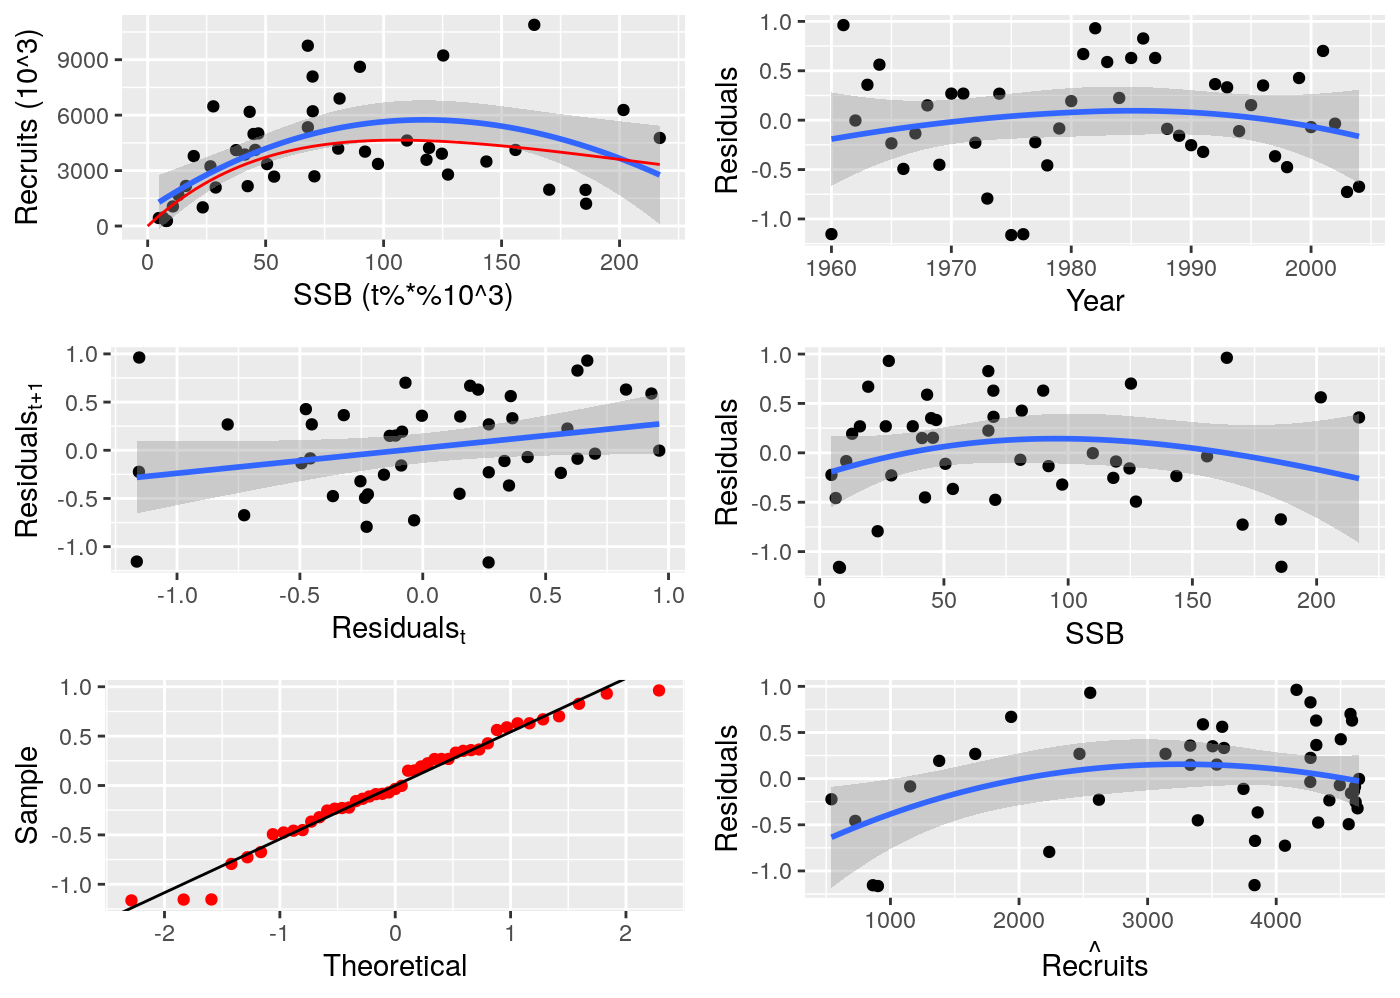
\includegraphics{SI5_files/figure-latex/unnamed-chunk-11-1.pdf}

We now have a working example of a stock-recruitment model, but for our
integration with \texttt{gmse\_apply}, we will want a function that
automates the above to simulate the process of updating the
stock-recruitment model. We do this using the custom function created
below.

\begin{Shaded}
\begin{Highlighting}[]
\NormalTok{update_SR_model <-}\StringTok{ }\NormalTok{function(rec_m, ssb_m, years)\{}
    \NormalTok{Frec_m       <-}\StringTok{ }\KeywordTok{FLQuant}\NormalTok{(rec_m, }\DataTypeTok{dimnames=}\KeywordTok{list}\NormalTok{(}\DataTypeTok{age =} \DecValTok{1}\NormalTok{, }\DataTypeTok{year =} \NormalTok{years));}
    \NormalTok{Fssb_m       <-}\StringTok{ }\KeywordTok{FLQuant}\NormalTok{(ssb_m, }\DataTypeTok{dimnames=}\KeywordTok{list}\NormalTok{(}\DataTypeTok{age =} \DecValTok{1}\NormalTok{, }\DataTypeTok{year =} \NormalTok{years));}
    \NormalTok{Frec_m@units <-}\StringTok{ "10^3"}\NormalTok{;}
    \NormalTok{Fssb_m@units <-}\StringTok{ "t*10^3"}\NormalTok{;}
    \KeywordTok{rec}\NormalTok{(newFL)   <-}\StringTok{ }\NormalTok{Frec.m;}
    \KeywordTok{ssb}\NormalTok{(newFL)   <-}\StringTok{ }\NormalTok{Fssb.m;}
    \KeywordTok{range}\NormalTok{(newFL) <-}\StringTok{ }\KeywordTok{c}\NormalTok{(}\DecValTok{0}\NormalTok{, years[}\DecValTok{1}\NormalTok{], }\DecValTok{0}\NormalTok{, years[}\KeywordTok{length}\NormalTok{(years)]);}
    \KeywordTok{model}\NormalTok{(newFL) <-}\StringTok{ }\KeywordTok{ricker}\NormalTok{();}
    \NormalTok{newFL        <-}\StringTok{ }\KeywordTok{fmle}\NormalTok{(newFL);}
    \KeywordTok{return}\NormalTok{(newFL);}
\NormalTok{\}}
\end{Highlighting}
\end{Shaded}

The above function will be used within another custom function to
predict the next time step of recruitment.

\begin{Shaded}
\begin{Highlighting}[]
\NormalTok{predict_recruitment <-}\StringTok{ }\NormalTok{function(rec_m, ssb_m, years, new_ssb)\{}
    \NormalTok{newFL <-}\StringTok{ }\KeywordTok{update_SR_model}\NormalTok{(rec_m, ssb_m, years);}
    \NormalTok{a     <-}\StringTok{ }\KeywordTok{params}\NormalTok{(newFL)[[}\DecValTok{1}\NormalTok{]] }\CommentTok{# Extract 'a' parameter of the Ricker model}
    \NormalTok{b     <-}\StringTok{ }\KeywordTok{params}\NormalTok{(newFL)[[}\DecValTok{2}\NormalTok{]] }\CommentTok{# Extract 'b' parameter of the Ricker model}
    \NormalTok{rec   <-}\StringTok{ }\NormalTok{a *}\StringTok{ }\NormalTok{new_ssb *}\StringTok{ }\KeywordTok{exp}\NormalTok{(-b *}\StringTok{ }\NormalTok{new_ssb); }\CommentTok{# Predict the new recruitment}
    \KeywordTok{return}\NormalTok{(rec)}
\NormalTok{\}}
\end{Highlighting}
\end{Shaded}

In \texttt{gmse\_apply}, we will use the \texttt{predict\_recruitment}
function above as the resource (i.e., operational) model. The
\texttt{new\_ssb} reads in the new spawning stock biomass, which will be
calculated from the built-in GMSE \texttt{user} model.

\section{\texorpdfstring{Integrating \texttt{predict\_recruitment} with
\texttt{gmse\_apply}}{Integrating predict\_recruitment with gmse\_apply}}\label{integrating-predict_recruitment-with-gmse_apply}

The \href{http://www.flr-project.org/}{FLR project} includes libraries
that can be used to
\href{http://www.flr-project.org/doc/An_introduction_to_MSE_using_FLR.html}{perform
a management strategy evaluation} (MSE) under fisheries-focused
observation, manager, and user models. We will not recreate
\href{http://www.flr-project.org/doc/An_introduction_to_MSE_using_FLR.html}{this
approach}, or integrate any other submodels into GMSE as was done for
the population model above, although such integration of submodels
should be possible using similar techniques. Our goal here is to instead
show how the \texttt{predict\_recruitment} model created above can be
integrated with \texttt{gmse\_apply}, which can then make use of the
genetic algorithm to predict the behaviour fishers.

We will use a custom observation model, which will simply estimate
recruitment with some fixed error.

\begin{Shaded}
\begin{Highlighting}[]
\NormalTok{obs_ssb <-}\StringTok{ }\NormalTok{function(resource_vector)\{}
    \NormalTok{obs_err <-}\StringTok{ }\KeywordTok{rnorm}\NormalTok{(}\DataTypeTok{n =} \DecValTok{1}\NormalTok{, }\DataTypeTok{mean =} \DecValTok{0}\NormalTok{, }\DataTypeTok{sd =} \DecValTok{100}\NormalTok{);}
    \NormalTok{the_obs <-}\StringTok{ }\NormalTok{resource_vector +}\StringTok{ }\NormalTok{obs_err;}
    \KeywordTok{return}\NormalTok{(the_obs);}
\NormalTok{\}}
\end{Highlighting}
\end{Shaded}

Hence, we can now feed the data from \texttt{rec.m} and \texttt{ssb.m}
through \texttt{predict\_recruitment}, which will return a value for new
recruitment, and this new value can in turn be fed into
\texttt{obs\_ssb} to predict recruitment with some error. We also need a
new spawning stock biomass \texttt{new\_ssb}, which we can just
initialise with the biomass from the last year in \texttt{ssb.m}

\begin{Shaded}
\begin{Highlighting}[]
\NormalTok{ssb_ini <-}\StringTok{ }\NormalTok{ssb.m[}\KeywordTok{length}\NormalTok{(ssb.m)];}
\NormalTok{new_rec <-}\StringTok{ }\KeywordTok{predict_recruitment}\NormalTok{(}\DataTypeTok{rec_m =} \NormalTok{rec.m, }\DataTypeTok{ssb_m =} \NormalTok{ssb.m, }\DataTypeTok{years =} \DecValTok{1960}\NormalTok{:}\DecValTok{2004}\NormalTok{,}
                               \DataTypeTok{new_ssb =} \NormalTok{ssb_ini);}
\NormalTok{obs_rec <-}\StringTok{ }\KeywordTok{obs_ssb}\NormalTok{(new_rec);}
\end{Highlighting}
\end{Shaded}

An initial run of these models gives values of 3835.21 for
\texttt{new\_rec} and 4025.16 for \texttt{obs\_rec}. We are now ready to
use the built-in manager and user submodels in \texttt{gmse\_apply}. We
will assume that managers attempt to keep a recruitment of 5000, and
that there are 4 independent fishers {[}stakehodlers in gmse\_apply says
10, is that a difference?{]} who attempt to maximise their catch. We
assign a user budget of \texttt{manager\_budget\ =\ 10000}, and all
other values are set to GMSE defaults. In the built-in GMSE functions,
the manager will use the estimate of recruitment based on
\texttt{obs\_rec} and use it to set the cost of harvesting
(\texttt{culling} in GMSE).

\begin{Shaded}
\begin{Highlighting}[]
\NormalTok{yrspan       <-}\StringTok{ }\DecValTok{1960}\NormalTok{:}\DecValTok{2004}\NormalTok{;}
\NormalTok{rec.m        <-}\StringTok{ }\KeywordTok{as.matrix}\NormalTok{(rec.n);}
\NormalTok{ssb.m        <-}\StringTok{ }\KeywordTok{as.matrix}\NormalTok{(ssb.n);}

\NormalTok{sim <-}\StringTok{ }\KeywordTok{gmse_apply}\NormalTok{(}\DataTypeTok{res_mod =} \NormalTok{predict_recruitment, }\DataTypeTok{obs_mod =} \NormalTok{obs_ssb,}
                  \DataTypeTok{rec_m =} \NormalTok{rec.m, }\DataTypeTok{ssb_m =} \NormalTok{ssb.m, }\DataTypeTok{years =} \NormalTok{yrspan, }
                  \DataTypeTok{new_ssb =} \NormalTok{ssb_ini, }\DataTypeTok{manage_target =} \DecValTok{5000}\NormalTok{, }\DataTypeTok{stakeholders =} \DecValTok{10}\NormalTok{,}
                  \DataTypeTok{manager_budget =} \DecValTok{10000}\NormalTok{);}
\KeywordTok{print}\NormalTok{(sim);}
\end{Highlighting}
\end{Shaded}

\begin{verbatim}
## $resource_results
## [1] 3835
## 
## $observation_results
## [1] 3617.956
## 
## $manager_results
##          resource_type scaring culling castration feeding help_offspring
## policy_1             1      NA     456         NA      NA             NA
## 
## $user_results
##         resource_type scaring culling castration feeding help_offspring
## Manager             1      NA       0         NA      NA             NA
## user_1              1      NA       2         NA      NA             NA
## user_2              1      NA       2         NA      NA             NA
## user_3              1      NA       2         NA      NA             NA
## user_4              1      NA       2         NA      NA             NA
## user_5              1      NA       2         NA      NA             NA
## user_6              1      NA       2         NA      NA             NA
## user_7              1      NA       2         NA      NA             NA
## user_8              1      NA       2         NA      NA             NA
## user_9              1      NA       2         NA      NA             NA
## user_10             1      NA       2         NA      NA             NA
##         tend_crops kill_crops
## Manager         NA         NA
## user_1          NA         NA
## user_2          NA         NA
## user_3          NA         NA
## user_4          NA         NA
## user_5          NA         NA
## user_6          NA         NA
## user_7          NA         NA
## user_8          NA         NA
## user_9          NA         NA
## user_10         NA         NA
\end{verbatim}

The resource and observation results above are interpreted in terms of
recruitment, while the manager results are interpreted in terms of the
cost of harvesting a unit of spawning stock biomass and the user results
are interpreted in terms of how much biomass was harvested. Note in the
run of \texttt{gmse\_apply} that the arguments for our custom resource
and observation models (\texttt{predict\_recruitment} and
\texttt{obs\_ssb}, respectively) are read directly in as arguments of
\texttt{gmse\_apply} itself. The \texttt{gmse\_apply} function will
figure out which subfunctions custom arguments should go to, then update
these arguments as needed over the course of a single run of
\texttt{gmse\_apply}.

\section{\texorpdfstring{Simulation with \texttt{gmse\_apply} over
multiple time
steps}{Simulation with gmse\_apply over multiple time steps}}\label{simulation-with-gmse_apply-over-multiple-time-steps}

We are now ready to loop the \texttt{gmse\_apply} function over multiple
time steps. To do this, we will update the \texttt{rec.m} and
\texttt{ssb.m} matrices after each time step, simulating 20 years into
the future. The population model \texttt{predict\_recruitment} will use
these data to dynamically update parameters of the Ricker model, as
might occur in an empirical fishery that is being monitored. We will use
the results from the observation model to update recruiment for the new
year in \texttt{rec.m}. For simplicity, spawning stock biomass prior to
harvest will be randomly sampled from a value in last 10 years (i.e.,
from \texttt{ssb.m} between 1994 and 2004), but more realistic models
could relate this spawning stock biomass to recruitment and
environmental variables from a prevoius year; spawning stock biomass
will be decreased after harvest based on user actions. The GMSE
initialisation and simulation is below.

\begin{Shaded}
\begin{Highlighting}[]
\CommentTok{# This code initialises the simulation -----------------------------------------}
\NormalTok{yrspan       <-}\StringTok{ }\DecValTok{1960}\NormalTok{:}\DecValTok{2004}\NormalTok{;}
\NormalTok{rec.m        <-}\StringTok{ }\KeywordTok{as.matrix}\NormalTok{(rec.n);}
\NormalTok{ssb.m        <-}\StringTok{ }\KeywordTok{as.matrix}\NormalTok{(ssb.n);}
\NormalTok{ssb_ini      <-}\StringTok{ }\NormalTok{ssb.m[}\KeywordTok{length}\NormalTok{(ssb.m)];}
\NormalTok{sim_old      <-}\StringTok{ }\KeywordTok{gmse_apply}\NormalTok{(}\DataTypeTok{res_mod =} \NormalTok{predict_recruitment, }\DataTypeTok{obs_mod =} \NormalTok{obs_ssb,}
                           \DataTypeTok{rec_m =} \NormalTok{rec.m, }\DataTypeTok{ssb_m =} \NormalTok{ssb.m, }\DataTypeTok{years =} \NormalTok{yrspan, }
                           \DataTypeTok{new_ssb =} \NormalTok{ssb_ini, }\DataTypeTok{manage_target =} \DecValTok{3500}\NormalTok{, }
                           \DataTypeTok{stakeholders =} \DecValTok{10}\NormalTok{, }\DataTypeTok{manager_budget =} \DecValTok{10000}\NormalTok{, }
                           \DataTypeTok{get_res =} \StringTok{"Full"}\NormalTok{);}
\CommentTok{# The code below simulates 20 time steps ---------------------------------------}
\NormalTok{sim_sum  <-}\StringTok{ }\KeywordTok{matrix}\NormalTok{(}\DataTypeTok{data =} \OtherTok{NA}\NormalTok{, }\DataTypeTok{nrow =} \DecValTok{20}\NormalTok{, }\DataTypeTok{ncol =} \DecValTok{6}\NormalTok{); }\CommentTok{# Hold results here}
\NormalTok{for(time_step in }\DecValTok{1}\NormalTok{:}\DecValTok{20}\NormalTok{)\{}
    \CommentTok{# Update the relevant parameter values as necessary -----------------------}
    \NormalTok{rand_ssb        <-}\StringTok{ }\KeywordTok{sample}\NormalTok{(}\DataTypeTok{x =} \NormalTok{ssb.m[}\DecValTok{35}\NormalTok{:}\DecValTok{45}\NormalTok{], }\DataTypeTok{size =} \DecValTok{1}\NormalTok{);}
    \NormalTok{harvest         <-}\StringTok{ }\KeywordTok{sum}\NormalTok{(sim_old$basic_output$user_results[,}\DecValTok{3}\NormalTok{]);}
    \NormalTok{new_rec_m       <-}\StringTok{ }\KeywordTok{c}\NormalTok{(sim_old$rec_m, sim_old$observation_vector);}
    \NormalTok{new_ssb_m       <-}\StringTok{ }\KeywordTok{c}\NormalTok{(sim_old$ssb_m, rand_ssb -}\StringTok{ }\NormalTok{harvest);}
    \NormalTok{sim_old$rec_m   <-}\StringTok{ }\KeywordTok{matrix}\NormalTok{(}\DataTypeTok{data =} \NormalTok{new_rec_m, }\DataTypeTok{nrow =} \DecValTok{1}\NormalTok{);}
    \NormalTok{sim_old$ssb_m   <-}\StringTok{ }\KeywordTok{matrix}\NormalTok{(}\DataTypeTok{data =} \NormalTok{new_ssb_m, }\DataTypeTok{nrow =} \DecValTok{1}\NormalTok{);}
    \NormalTok{sim_old$years   <-}\StringTok{ }\KeywordTok{c}\NormalTok{(sim_old$years, time_step +}\StringTok{ }\DecValTok{2004}\NormalTok{);}
    \NormalTok{sim_old$new_ssb <-}\StringTok{ }\NormalTok{sim_old$ssb_m[}\KeywordTok{length}\NormalTok{(sim_old$ssb_m)];}
    \CommentTok{# Run a new simulation in the loop: custom functions are always specified -}
    \NormalTok{sim_new  <-}\StringTok{ }\KeywordTok{gmse_apply}\NormalTok{(}\DataTypeTok{get_res =} \StringTok{"Full"}\NormalTok{, }\DataTypeTok{old_list =} \NormalTok{sim_old,}
                           \DataTypeTok{res_mod =} \NormalTok{predict_recruitment, }\DataTypeTok{obs_mod =} \NormalTok{obs_ssb);}
    \CommentTok{# Record the results in sim_sum -------------------------------------------}
    \NormalTok{sim_sum[time_step, }\DecValTok{1}\NormalTok{] <-}\StringTok{ }\NormalTok{time_step +}\StringTok{ }\DecValTok{2004}\NormalTok{;}
    \NormalTok{sim_sum[time_step, }\DecValTok{2}\NormalTok{] <-}\StringTok{ }\NormalTok{sim_new$basic_output$resource_results[}\DecValTok{1}\NormalTok{];}
    \NormalTok{sim_sum[time_step, }\DecValTok{3}\NormalTok{] <-}\StringTok{ }\NormalTok{sim_new$basic_output$observation_results[}\DecValTok{1}\NormalTok{];}
    \NormalTok{sim_sum[time_step, }\DecValTok{4}\NormalTok{] <-}\StringTok{ }\NormalTok{sim_new$basic_output$manager_results[}\DecValTok{3}\NormalTok{];}
    \NormalTok{sim_sum[time_step, }\DecValTok{5}\NormalTok{] <-}\StringTok{ }\NormalTok{harvest;}
    \NormalTok{sim_sum[time_step, }\DecValTok{6}\NormalTok{] <-}\StringTok{ }\NormalTok{sim_new$new_ssb;}
    \CommentTok{# Redefine the old list --------------------------------------------------}
    \NormalTok{sim_old               <-}\StringTok{ }\NormalTok{sim_new;}
\NormalTok{\}}
\KeywordTok{colnames}\NormalTok{(sim_sum) <-}\StringTok{ }\KeywordTok{c}\NormalTok{(}\StringTok{"Year"}\NormalTok{, }\StringTok{"Recruitment"}\NormalTok{, }\StringTok{"Recruit_estim"}\NormalTok{, }\StringTok{"Harvest_cost"}\NormalTok{, }
                         \StringTok{"Harvested"}\NormalTok{, }\StringTok{"SSB"}\NormalTok{);}
\KeywordTok{print}\NormalTok{(sim_sum);}
\end{Highlighting}
\end{Shaded}

\begin{verbatim}
##       Year Recruitment Recruit_estim Harvest_cost Harvested      SSB
##  [1,] 2005        4491      4535.352          478        20 135.9025
##  [2,] 2006        4647      4709.264          538        20 105.2627
##  [3,] 2007        4629      4821.850          583        10 115.2627
##  [4,] 2008        4387      4255.025          594        10 145.9025
##  [5,] 2009        3035      3078.288          636        10  35.5913
##  [6,] 2010        3035      3219.448          502        10  35.5913
##  [7,] 2011        4629      4685.483          613        10 115.2627
##  [8,] 2012        4629      4614.816          473        10 115.2627
##  [9,] 2013        2399      2365.097          530        20  25.5913
## [10,] 2014        2994      2930.048          486        10  34.8673
## [11,] 2015        2347      2336.880          530        20  24.8673
## [12,] 2016        3303      3357.941          492        10  40.6133
## [13,] 2017        4336      4227.214          523        20 150.1926
## [14,] 2018        4387      4401.982          513        10 145.9025
## [15,] 2019        4328      4356.673          544        10  70.7603
## [16,] 2020        3035      2979.304          546        10  35.5913
## [17,] 2021        4339      4457.722          536        10  71.3340
## [18,] 2022        4339      4319.507          557        10  71.3340
## [19,] 2023        4339      4490.953          523        10  71.3340
## [20,] 2024        3303      3274.942          473        10  40.6133
\end{verbatim}

The above output from \texttt{sim\_sum} reports the recruitment
(resource or operational model), recruitment estimate (observation error
model), management set harvest cost (harvest control model), user
harvested numbers (implementation model) and spawning stock biomass
(SSB) simulation results. This example simulation demonstrates the
ability of GMSE to integrate with fisheries libraries such as
\href{http://www.flr-project.org/}{FLR} through \texttt{gmse\_apply}. In
addition to being a useful wrapping function for MSE submodels,
\texttt{gmse\_apply} can therefore be used to take advantage of the
genetic algorithm in the GMSE default manager and user models. This
flexibility will be retained in future versions of \texttt{gmse\_apply},
allowing custom resource and observation models that are built for
specific systems to be integrated with an increasingly complex genetic
algorithm simulating various aspects of human decision-making.

\section{Conclusions}\label{conclusions}

GMSE is a general, flexible, tool for simulating the management of
resources under situations of uncertainty and conflict. Management
Strategy Evaluation \citep{Bunnefeld2011, Punt2016}, the framework upon
which GMSE is based, had its origin in fisheries management
\citep{Polacheck1999, Smith1999, Sainsbury2000}, and here we showed one
example of how GMSE could be integrated with the core package of the
\href{http://www.flr-project.org/}{Fisheries Library in R}.

Future versions of GMSE will continue to be open-source and developed to
avoid unecessary dependencies (GMSE v.0.4.0.3 requires only base R). Key
goals including (1) providing highly general and useful default
\texttt{resource}, \texttt{observation}, \texttt{manager}, and
\texttt{user} submodels for a variety of MSE modelling tasks, (2)
keeping these submodels highly modular so that they can be developed in
isolation given standardised data structures, and (3) allowing these
modular submodels to be integrated with custom defined submodels as
flexibly as possible using \texttt{gmse\_apply}. Contributions in line
with these goals, and suggestions for new features, can be made on
\href{https://github.com/bradduthie/gmse}{GitHub}.

\bibliography{gmse.bib}


\end{document}
